\cleardoublepage
\chapter{PERANCANGAN}
\label{chap:perancangan}

Bab ini memaparkan perancangan solusi yang menjawab kebutuhan pada Bab~\ref{chap:analisis-masalah}. Perancangan disajikan berurutan dari arsitektur umum (perbandingan \emph{before}--\emph{after} terhadap kondisi saat ini), batas penalaran mesin prakiraan beserta alasan pembatasannya, pipeline RAG \emph{terkondisi-prediksi} sebagai inti kebaruan, perancangan perangkat lunak (struktur kelas dan interaksi antarobjek), hingga perancangan antarmuka pengguna.

\section{Arsitektur Umum Solusi}
\label{sec:arsitektur-umum}
Arsitektur solusi mengubah alur reaktif pada Gambar~\ref{fig:alur-perawatan} menjadi alur \textbf{antisipatif} yang menghubungkan prediksi dengan pengetahuan klinis. Data \emph{logbook} tidak lagi berhenti sebagai catatan pasif yang ditafsirkan manual, melainkan mengalir melalui lapisan prediksi, lapisan \emph{state digital twin}, dan lapisan penalaran berbasis dokumen, hingga menghasilkan rekomendasi tertelusur yang divalidasi dokter. Gambar~\ref{fig:arsitektur} menyajikan arsitektur berlapis tersebut.

\begin{figure}[htbp]
\centering
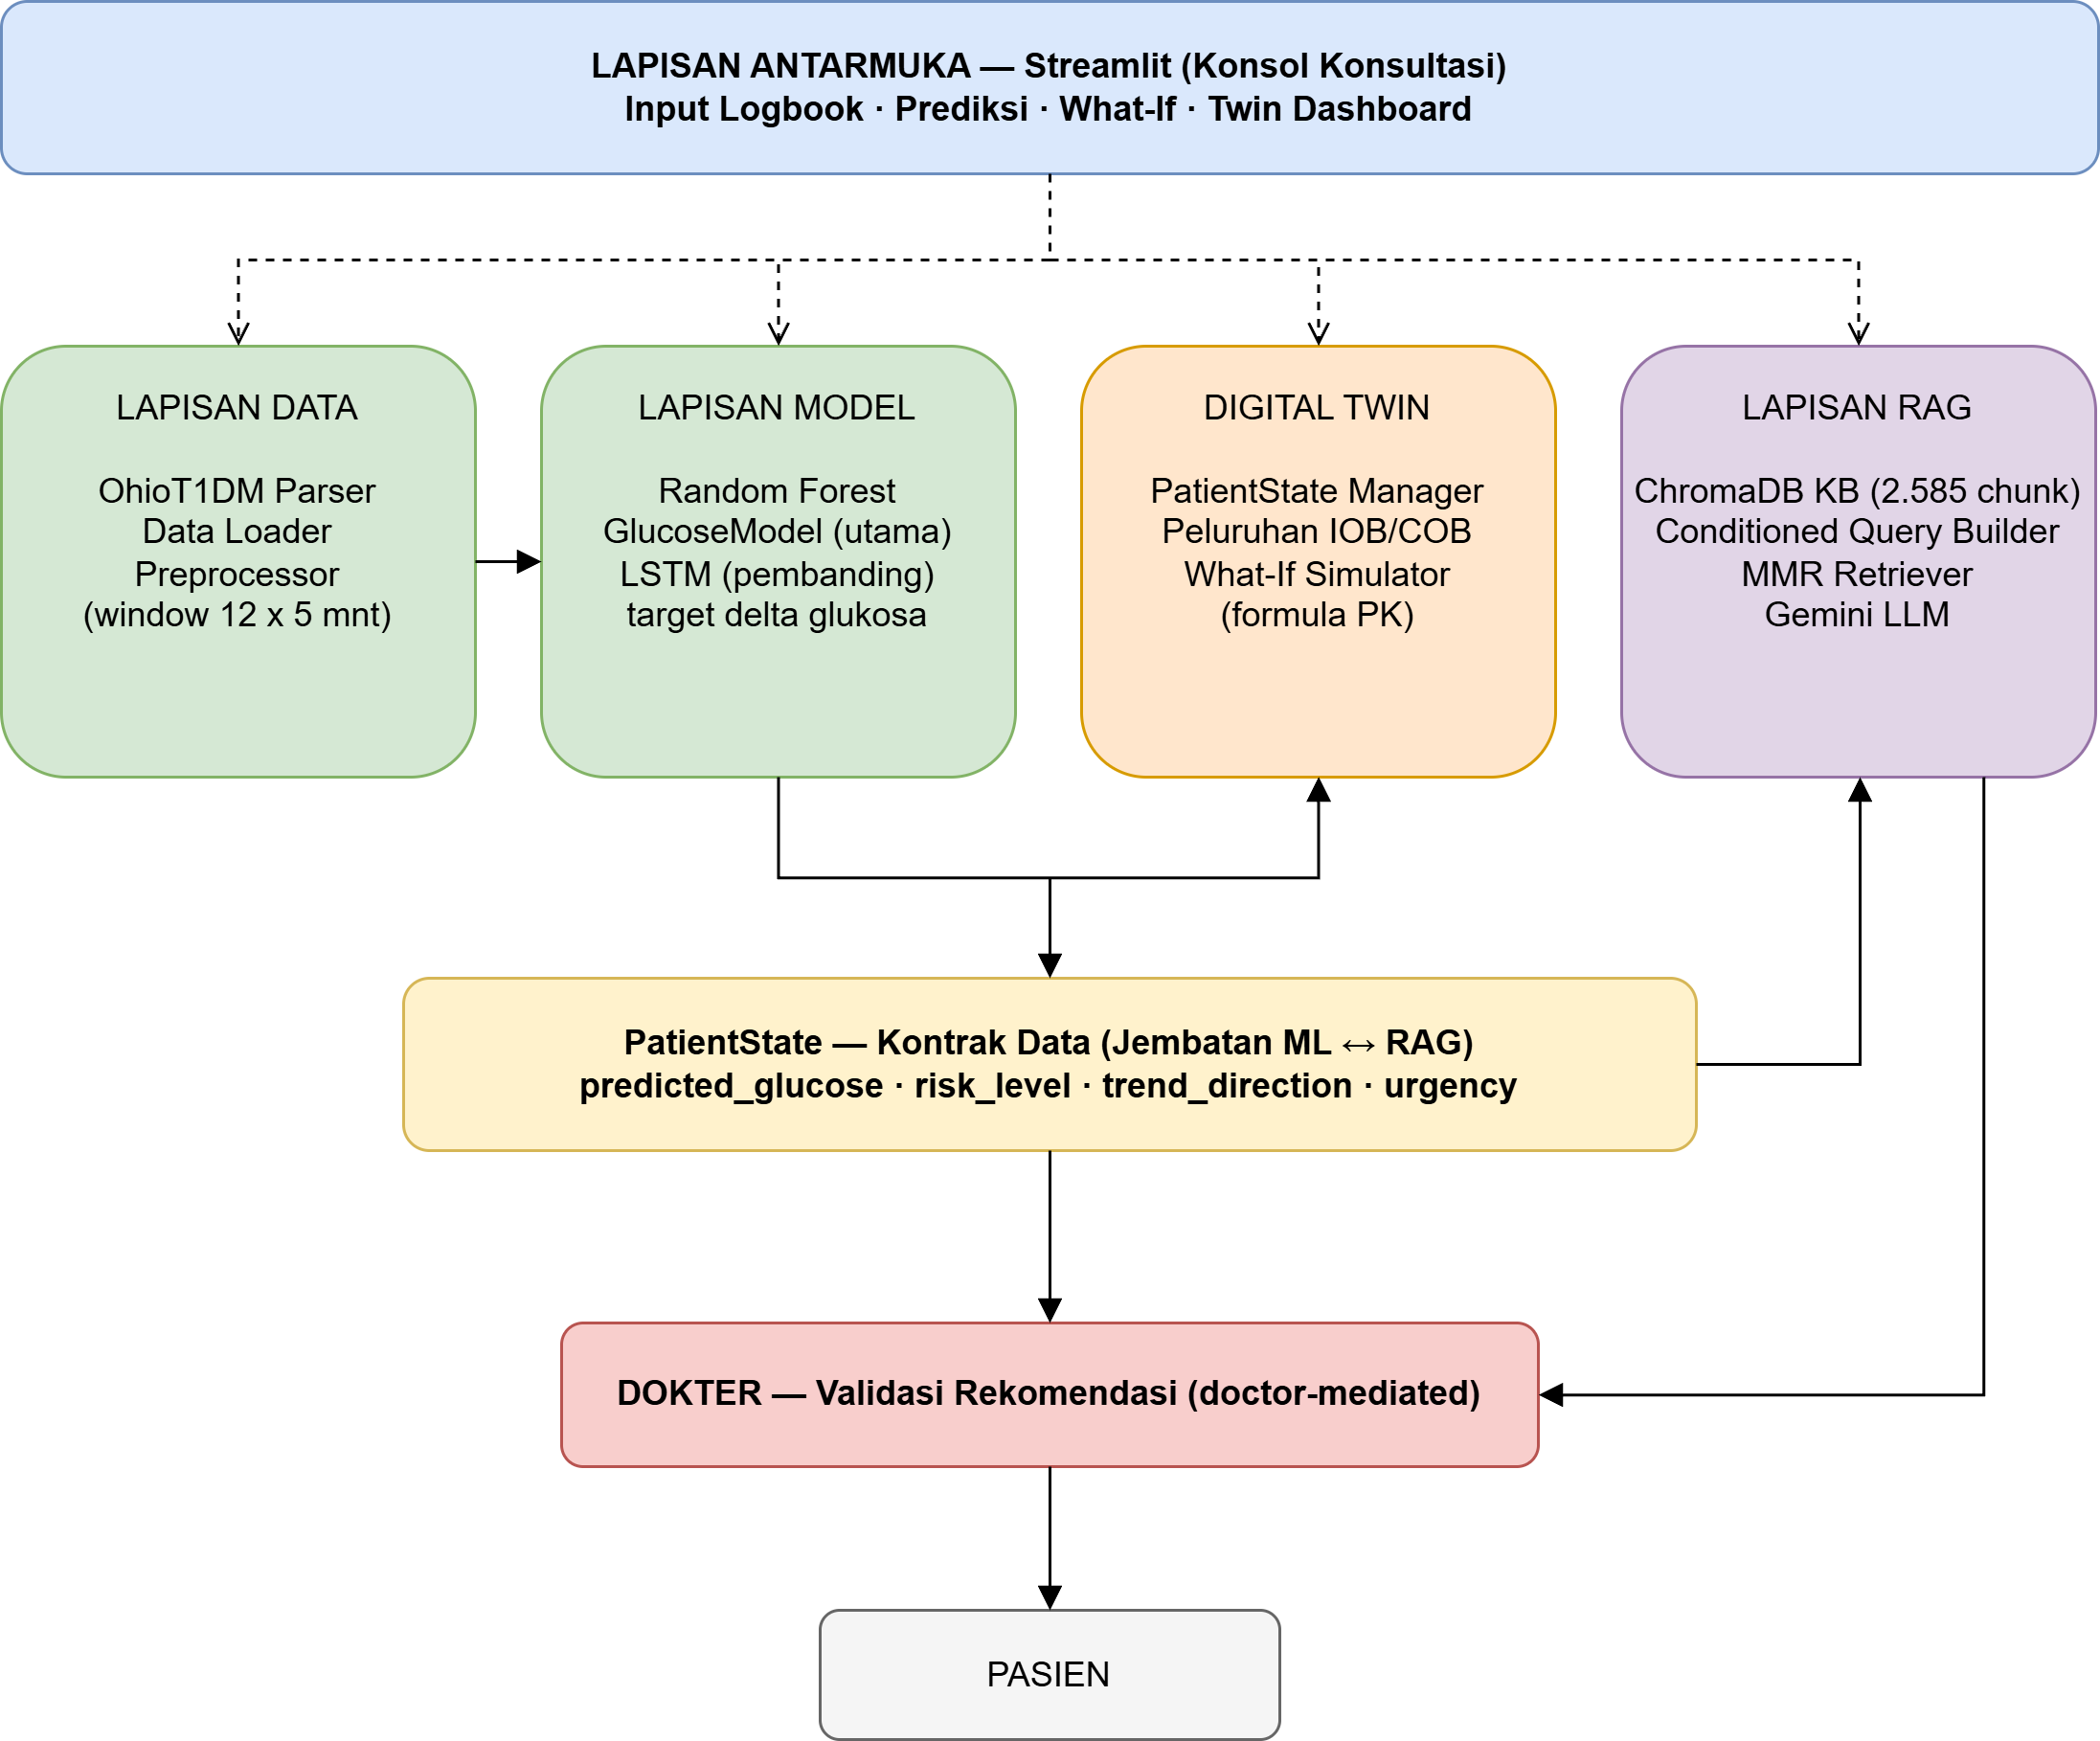
\includegraphics[width=0.95\textwidth]{images/Gambar_IV1_Arsitektur.png}
\caption{Arsitektur berlapis solusi: dari data \emph{logbook} menuju prediksi, \emph{state digital twin}, penalaran berbasis dokumen, dan rekomendasi tertelusur yang divalidasi dokter.}
\label{fig:arsitektur}
\end{figure}

Perbedaan mendasar terhadap kondisi saat ini dirangkum sebagai berikut. \emph{Pertama}, titik masalah ``reaktif'' digantikan modul prediksi glukosa jangka pendek yang menatap ke depan ($+30/+60$ menit). \emph{Kedua}, ``interpretasi manual'' dibantu \emph{state digital twin} yang meringkas tingkat risiko, arah tren, dan urgensi. \emph{Ketiga}, ``prediksi terputus dari rekomendasi'' dijembatani mekanisme RAG \emph{terkondisi-prediksi} yang menjadikan nilai terprediksi sebagai konteks kueri. \emph{Keempat}, seluruh infrastruktur dirancang \emph{deployable} tanpa GPU, CGM \emph{real-time}, maupun EHR, sehingga selaras dengan kendala FKTP dan berbeda dari kerangka berbasis \emph{knowledge graph} yang menuntut infrastruktur berat \autocite{rad2024}.

\section{Batas Penalaran Mesin Prakiraan}
\label{sec:batas-prakiraan}
Sistem memiliki \textbf{satu} mesin komputasi, yaitu \textbf{mesin prakiraan}, yang menjawab pertanyaan \emph{``apa yang akan terjadi?''} dengan memetakan \emph{state} fisiologis terkini ke $\Delta$glukosa pada horizon tetap menggunakan model \emph{Gradient Boosting}. Sistem \textbf{sengaja tidak} menjawab pertanyaan \emph{``apa yang terjadi jika dokter mengubah insulin atau karbohidrat?''}. Pembatasan itu merupakan keputusan perancangan yang berdasar, bukan fitur yang belum sempat dibuat.

Alasannya terletak pada sifat model yang dipakai. Model \emph{Gradient Boosting} bersifat \textbf{korelasional}, bukan kausal. Pada data latih, insulin diberikan \emph{karena} glukosa sedang tinggi, sehingga asosiasi yang dipelajari model adalah ``dosis insulin besar muncul bersama glukosa tinggi''. Bila model yang sama dipakai untuk mensimulasikan tindakan ``menambah insulin'', ia akan mengikuti asosiasi tersebut dan menghasilkan arah kontrafaktual yang \textbf{terbalik dari kenyataan fisiologisnya}. Keluaran seperti itu berbahaya justru karena tampak masuk akal: angkanya wajar, arahnya salah, dan kesalahannya tidak terlihat dari metrik regresi mana pun.

Menyediakan simulasi intervensi karena itu menuntut model mekanistik yang menegakkan arah kausal secara eksplisit, misalnya formula farmakokinetik. Membangun dan memvalidasi model semacam itu berada di luar cakupan tugas akhir ini, dan menyajikannya tanpa validasi klinis akan bertentangan dengan Batasan~4 yang menempatkan sistem sebagai pendukung keputusan ber-alur \emph{doctor-mediated}, bukan penentu tindakan.

Konsekuensinya terhadap alur kerja bersifat mendasar dan disengaja: sistem menyajikan \textbf{prakiraan beserta pedoman yang relevan terhadap kondisi yang diprakirakan}, sedangkan pemilihan intervensi tetap sepenuhnya berada pada dokter. Pembagian peran itu sejalan dengan rancangan \emph{human-in-the-loop} pada Subbab~\ref{sec:arsitektur-umum} dan menjadi dasar tinjauan dokter sebelum keputusan dicatat.

\section{Perancangan Pipeline RAG \emph{terkondisi-prediksi}}
Inti kebaruan tugas akhir ini adalah pipeline RAG \emph{terkondisi-prediksi} pada Gambar~\ref{fig:pipeline-pcrag}. Berbeda dari RAG standar yang menyusun kueri hanya dari kondisi \emph{terkini}, RAG terkondisi-prediksi menyisipkan hasil prediksi ke dalam pembentukan kueri sehingga \emph{retrieval} diarahkan pada dokumen yang relevan terhadap kondisi yang \emph{akan datang}.

\begin{figure}[htbp]
\centering
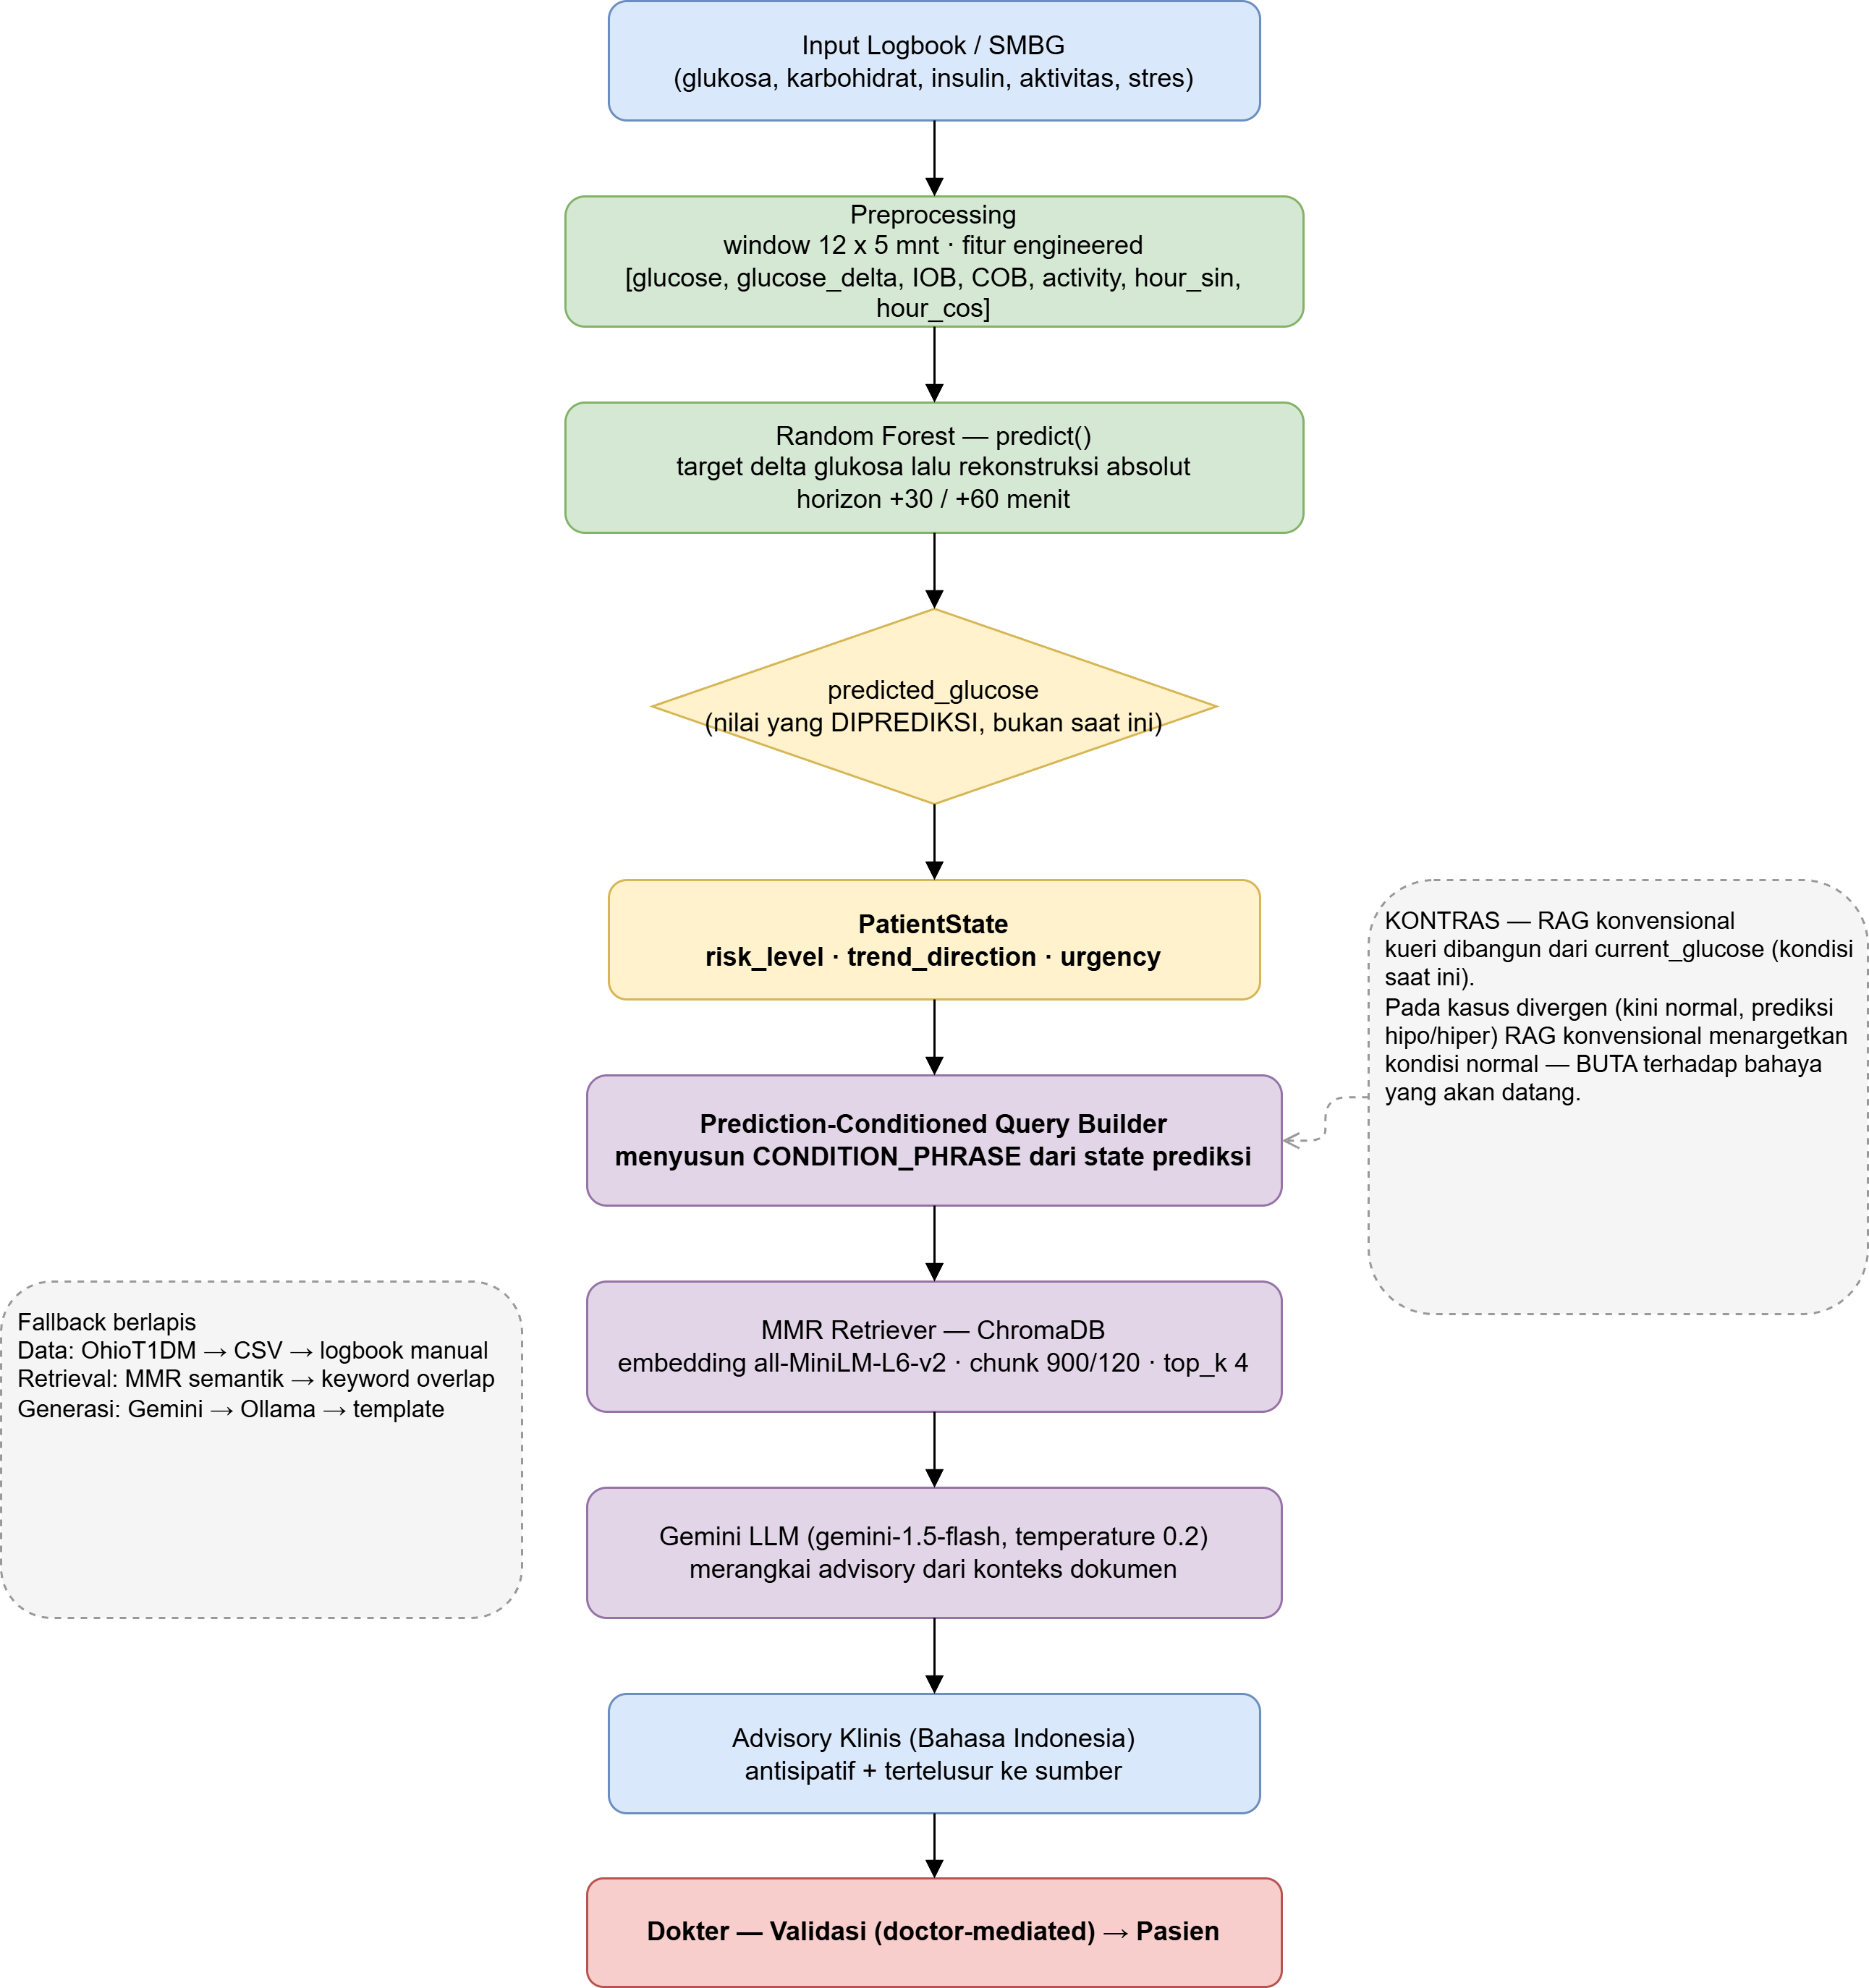
\includegraphics[width=0.95\textwidth]{images/Gambar_IV3_PipelinePCRAG.png}
\caption{Pipeline RAG \emph{terkondisi-prediksi}: nilai glukosa terprediksi mengondisikan pembentukan kueri \emph{retrieval} sebelum generasi rekomendasi.}
\label{fig:pipeline-pcrag}
\end{figure}

Alur pipeline: (1)~\emph{state} fisiologis terkini diekstraksi dari \emph{logbook}; (2)~model \emph{Random Forest} memprediksi glukosa $+30/+60$ menit; (3)~nilai terprediksi diklasifikasikan menjadi kondisi klinis (hipoglikemia/normal/hiperglikemia) dan digabung dengan konteks terkini untuk membentuk \textbf{kueri yang dikondisikan prediksi}; (4)~kueri di-\emph{embed} dengan \texttt{all-MiniLM-L6-v2} dan dipakai untuk \emph{retrieval} dari basis pengetahuan klinis pada ChromaDB; (5)~potongan dokumen teratas diberikan sebagai konteks kepada LLM \textbf{\texttt{gemini-2.5-flash-lite}} dengan parameter generatif konservatif; (6)~LLM menghasilkan rekomendasi berbahasa Indonesia yang \emph{grounded} dan tertelusur. Setiap lapisan dilengkapi \emph{graceful fallback} agar sistem tetap memberi keluaran aman saat salah satu komponen gagal.

\section{Perancangan Perangkat Lunak}
Perangkat lunak dirancang memisahkan \emph{domain logic} dari antarmuka (KNF-07) agar mudah dipelihara. Struktur kelas utama, meliputi pemuat data, prediktor, \emph{engine} \emph{digital twin}, \emph{retriever}, dan generator rekomendasi, ditunjukkan pada Gambar~\ref{fig:class-diagram}.

\begin{figure}[htbp]
\centering
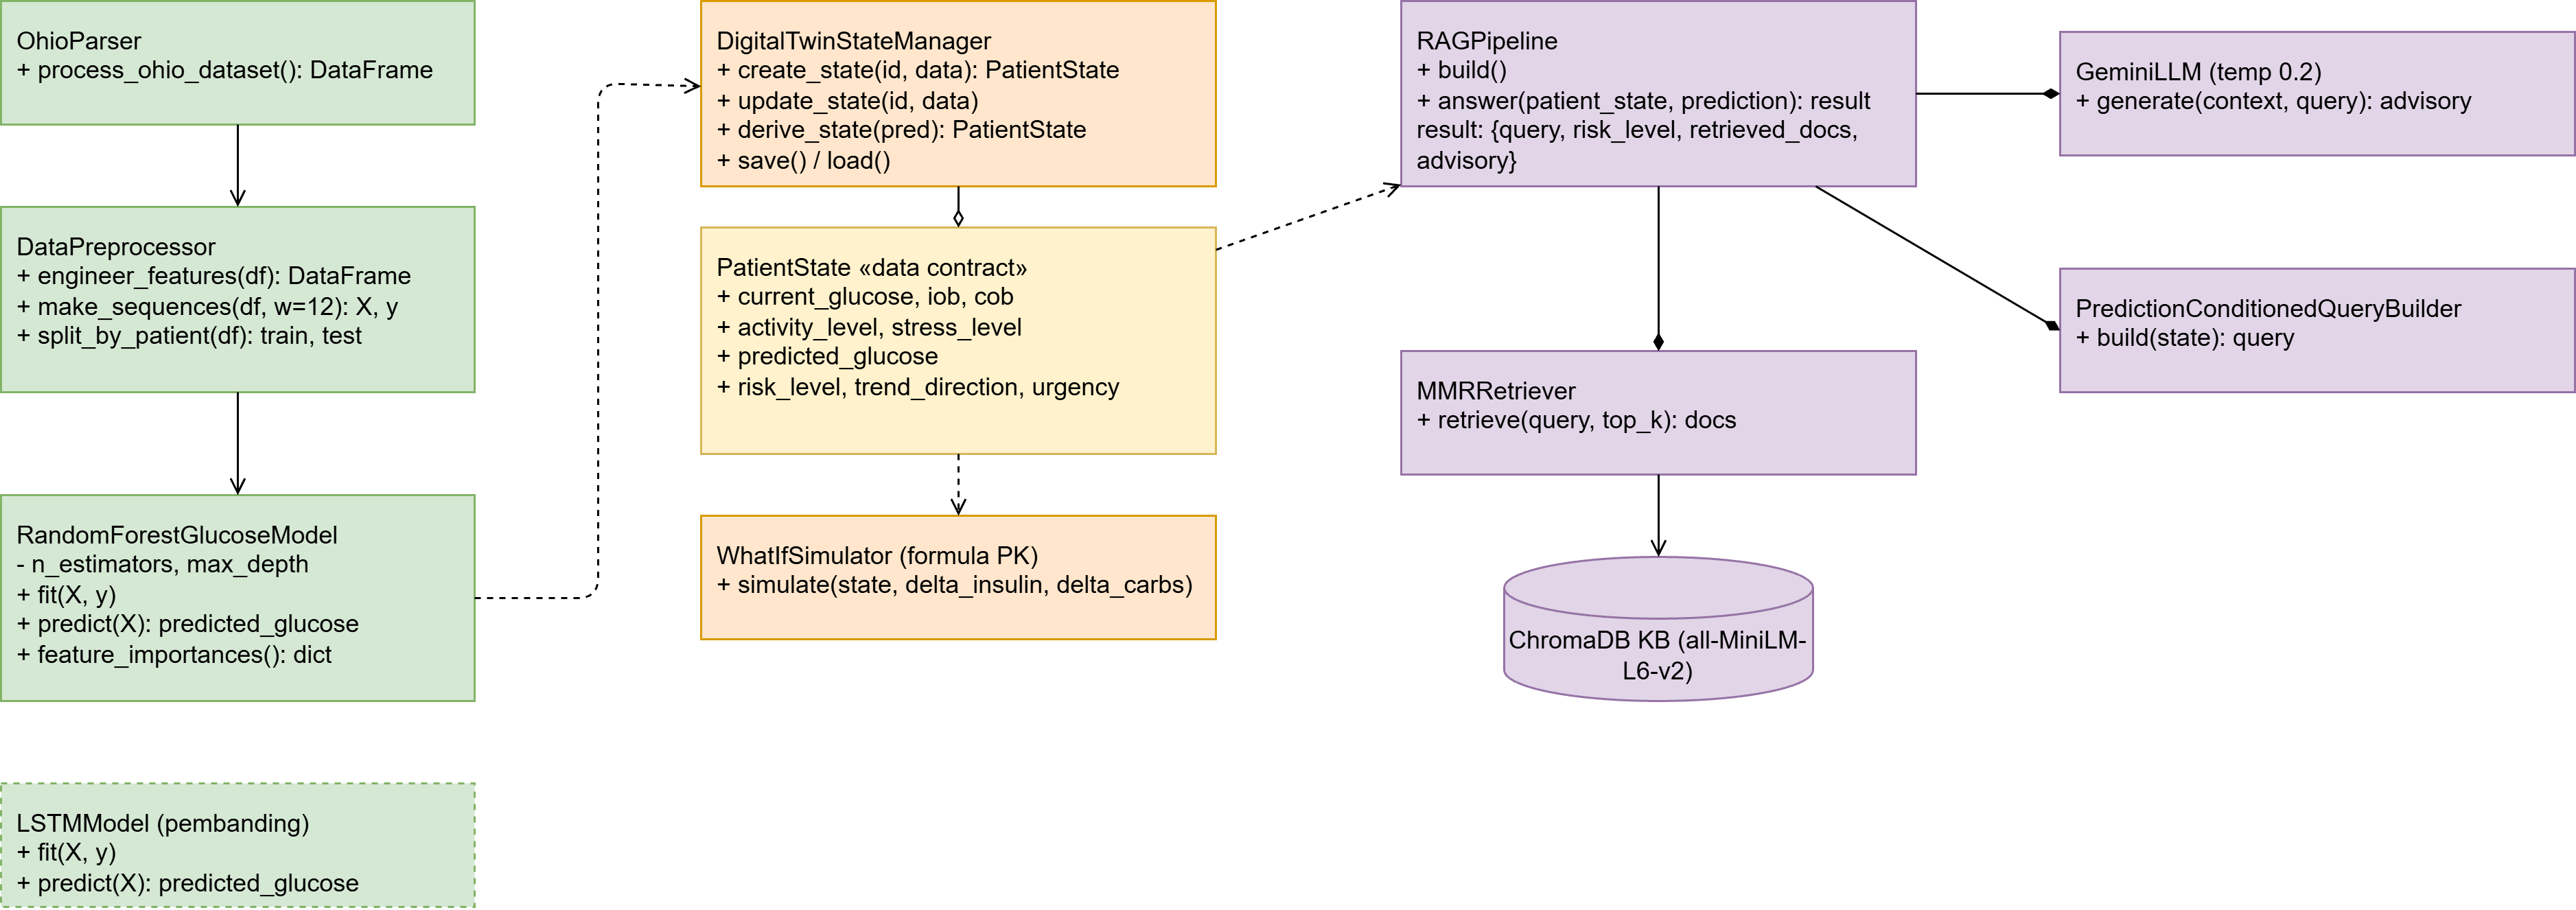
\includegraphics[width=0.95\textwidth]{images/Gambar_IV4_ClassDiagram.png}
\caption{Diagram kelas komponen inti sistem, memisahkan \emph{domain logic} (prediksi, \emph{digital twin}, \emph{retrieval}, generasi) dari lapisan antarmuka.}
\label{fig:class-diagram}
\end{figure}

Interaksi antarobjek saat menjalankan satu siklus RAG terkondisi-prediksi, dari permintaan dokter hingga rekomendasi tertelusur, ditunjukkan pada diagram sekuens Gambar~\ref{fig:sequence-pcrag}.

\begin{figure}[htbp]
\centering
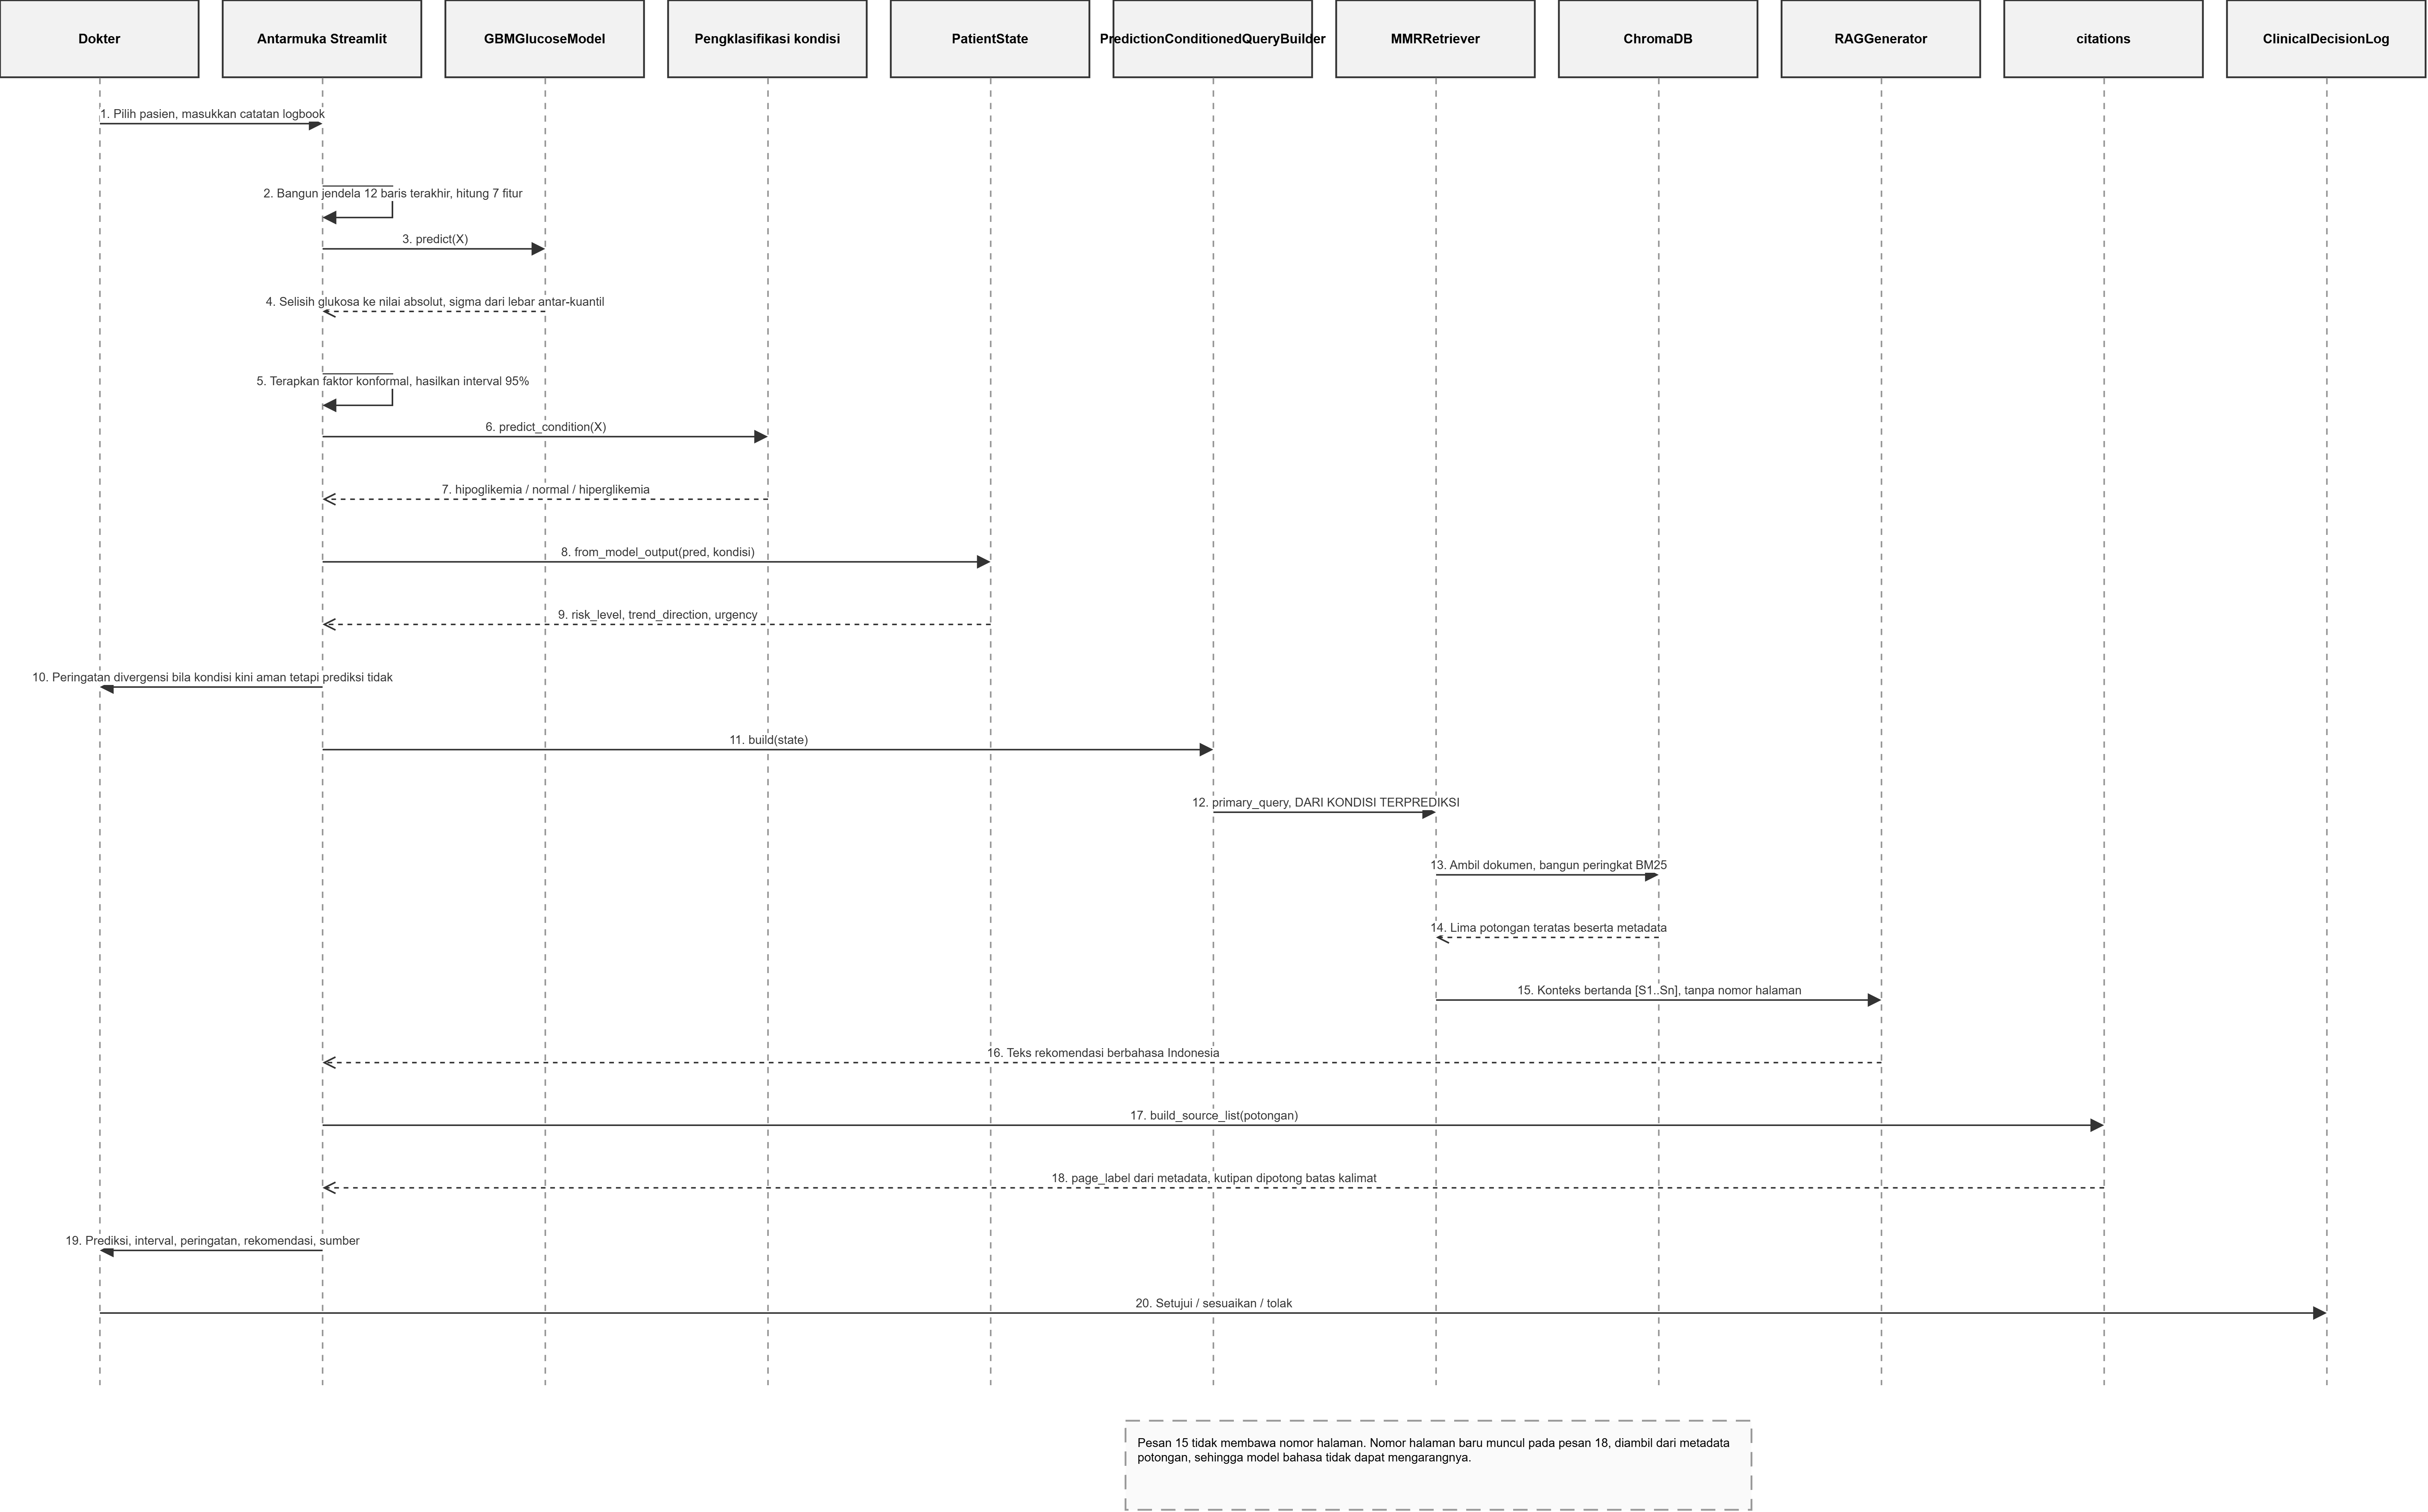
\includegraphics[width=0.95\textwidth]{images/Gambar_IV5_SequencePCRAG.png}
\caption{Diagram sekuens satu siklus RAG \emph{terkondisi-prediksi}, dari permintaan dokter hingga rekomendasi tertelusur.}
\label{fig:sequence-pcrag}
\end{figure}

\section{Perancangan Antarmuka Pengguna}
Antarmuka dirancang sebagai alat konsultasi klinis \emph{multi-page} berbasis Streamlit untuk dokter, dengan panel \emph{state digital twin}, penyajian prediksi beserta interval ketidakpastian, \emph{slider what-if} untuk simulasi intervensi, dan rekomendasi tertelusur ke dokumen sumber. Rancangan \emph{wireframe} antarmuka ditunjukkan pada Gambar~\ref{fig:wireframe}. Alur \emph{doctor-mediated} (KF-09) diwujudkan melalui langkah validasi eksplisit sebelum rekomendasi diteruskan kepada pasien.

\begin{figure}[htbp]
\centering
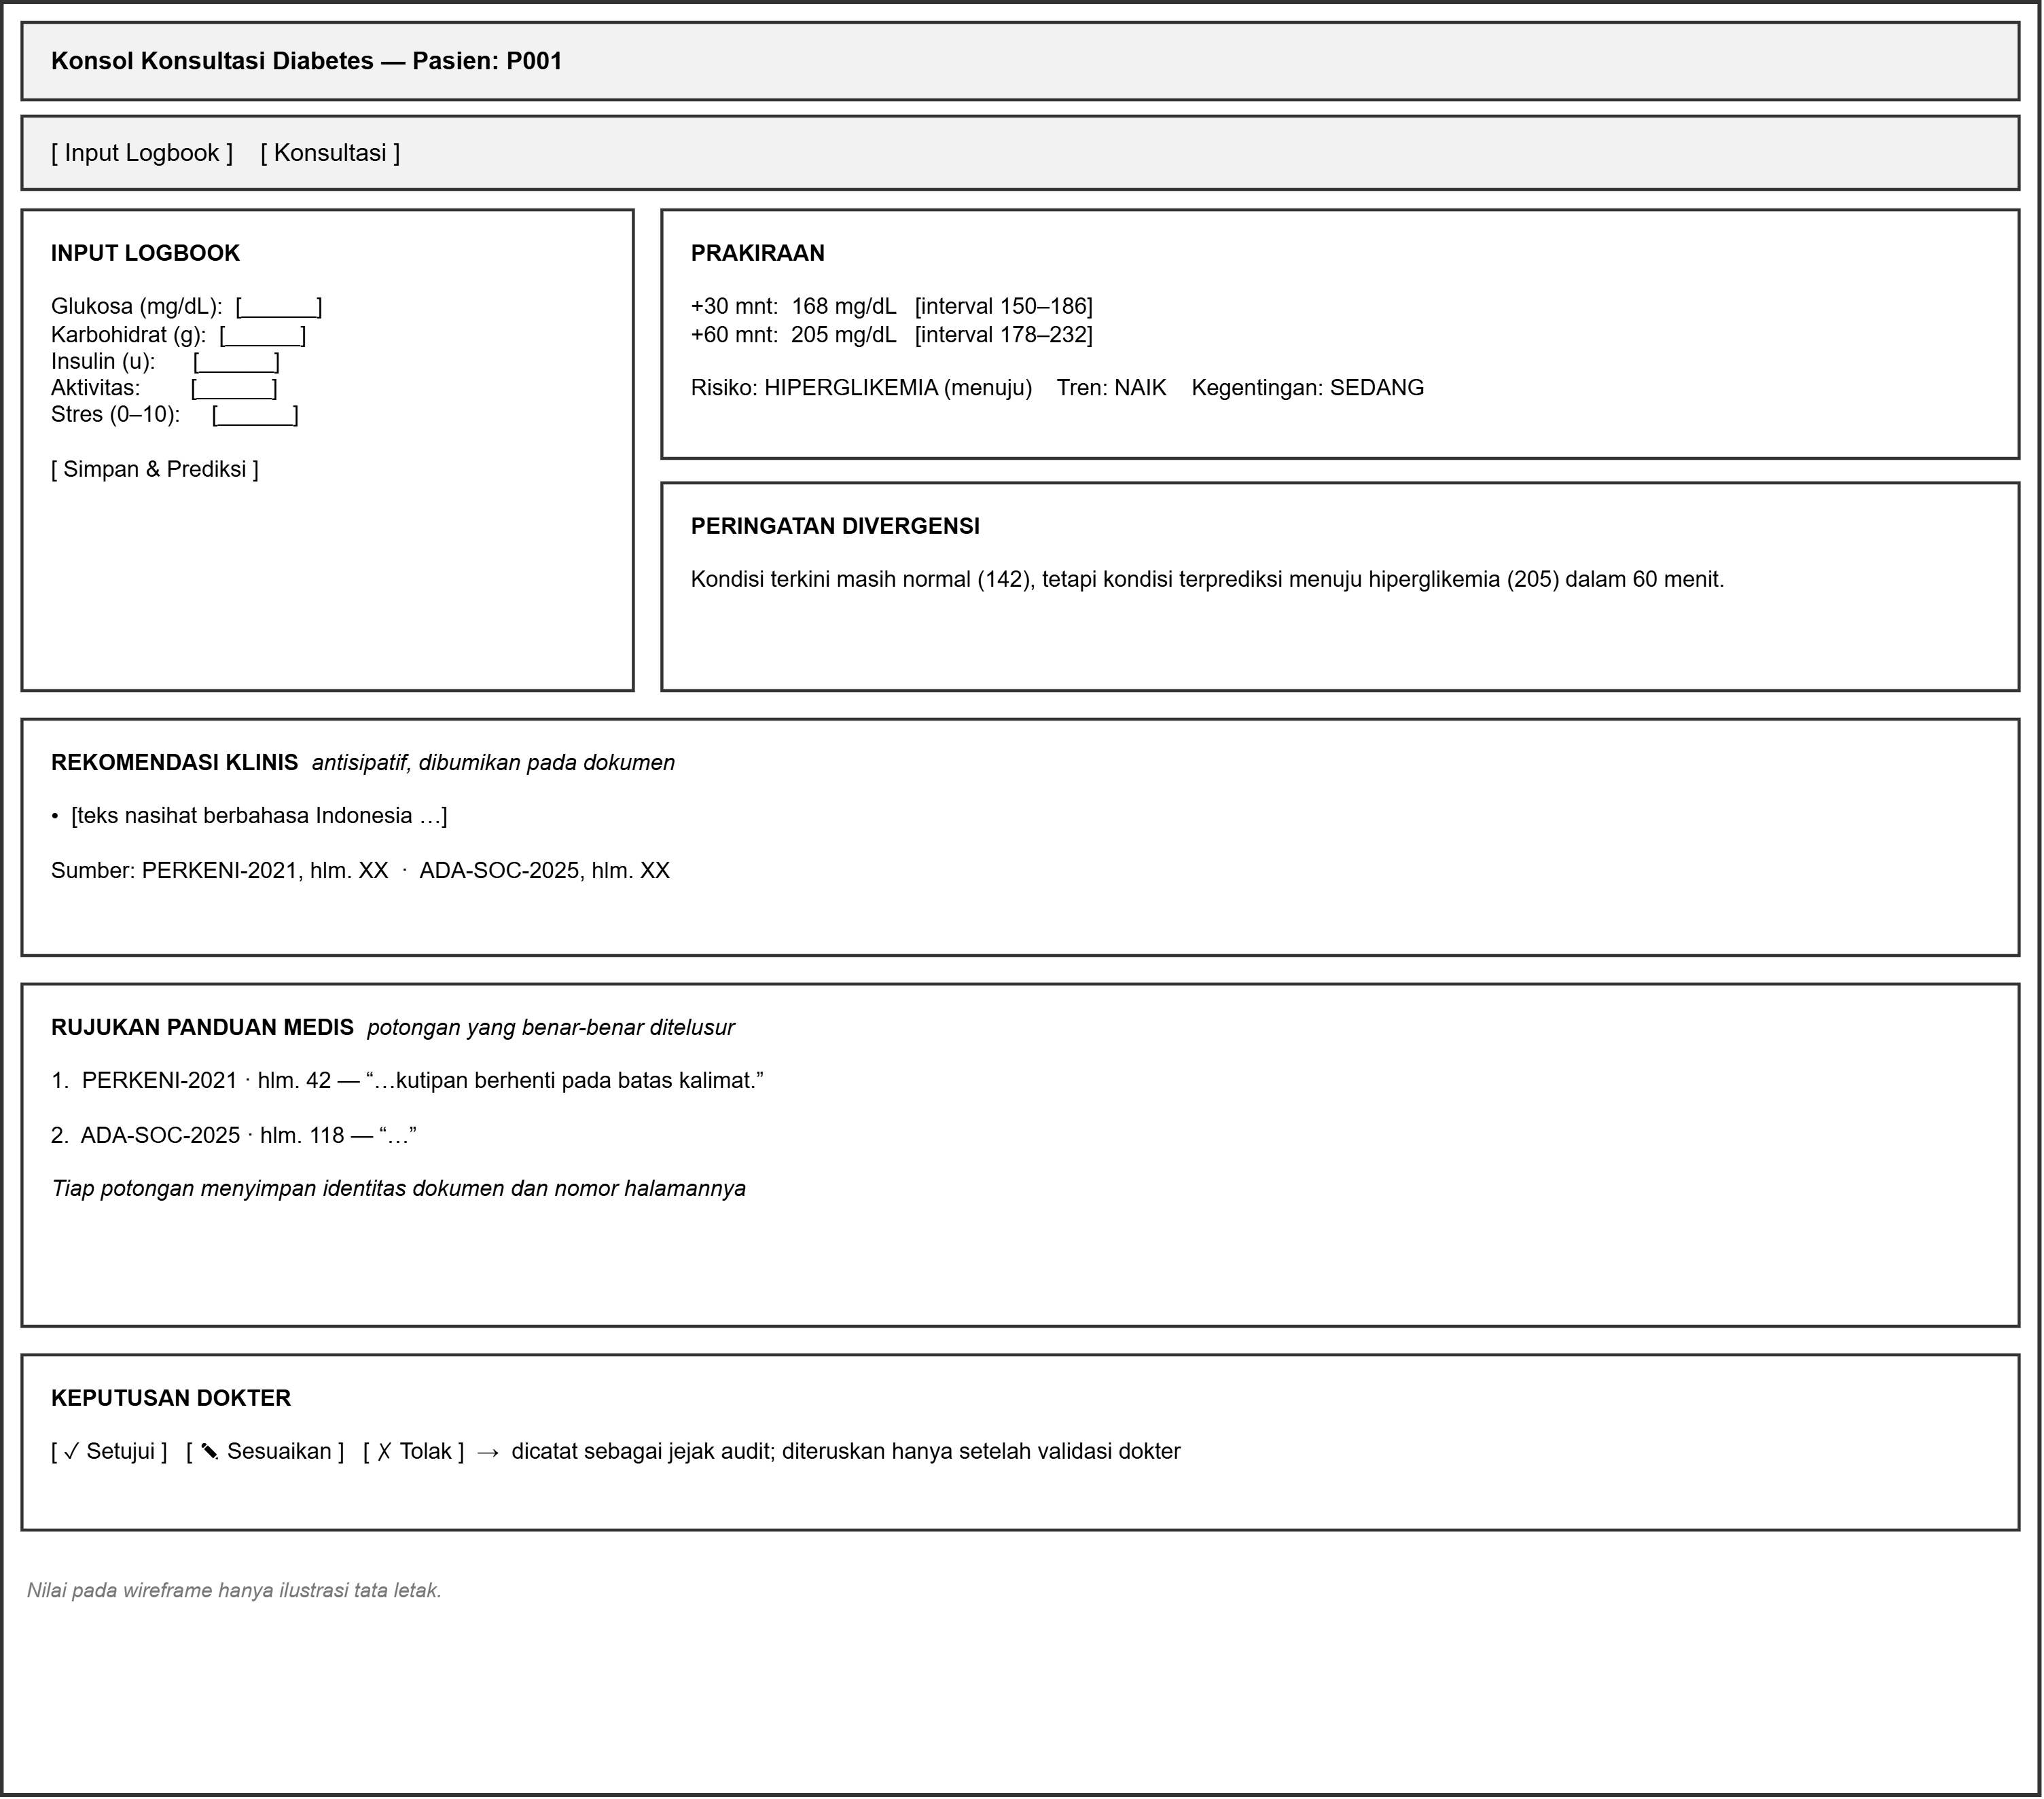
\includegraphics[width=0.95\textwidth]{images/Gambar_IV6_Wireframe.png}
\caption{Rancangan \emph{wireframe} antarmuka alat konsultasi klinis: panel \emph{state digital twin}, prediksi dengan interval, \emph{slider what-if}, dan rekomendasi tertelusur.}
\label{fig:wireframe}
\end{figure}
